% Template:     Informe LaTeX
% Documento:    Archivo de ejemplo
% Versión:      8.3.6 (23/08/2024)
% Codificación: UTF-8
%
% Autor: Pablo Pizarro R.
%        pablo@ppizarror.com
%
% Manual template: [https://latex.ppizarror.com/informe]
% Licencia MIT:    [https://opensource.org/licenses/MIT]

% ------------------------------------------------------------------------------
% NUEVA SECCIÓN
% ------------------------------------------------------------------------------
% Las secciones se inician con \section, si se quiere una sección sin número se
% pueden usar las funciones \sectionanum (sección sin número) o la función
% \sectionanumnoi para crear el mismo título sin numerar y sin aparecer en el índice
\section{Introducción}
El Laboratorio de Ondas Milimétricas (MWL) de la Universidad de Chile, es un centro dedicado al diseño y construcción, diseño y diferentes elementos para aplicaciones en radioastronomía, y otras areas de la ingeneria segun sea el proyecto que adquieran. Este laboratorio se destaca por su enfoque en la investigación tecnológica avanzada y colabora en proyectos internacionales de gran relevancia, particularmente en el campo de la observación astronómica y microondas. El MWL está compuesto por un equipo multidisciplinario de astrónomos, ingenieros y estudiantes (\ref{fig:personas_lab}), quienes combinan sus conocimientos para llevar a cabo estudios de frecuencias que abarcan desde el espectro decamétrico hasta el submilimétrico.\\\\
\begin{figure}
	\centering
	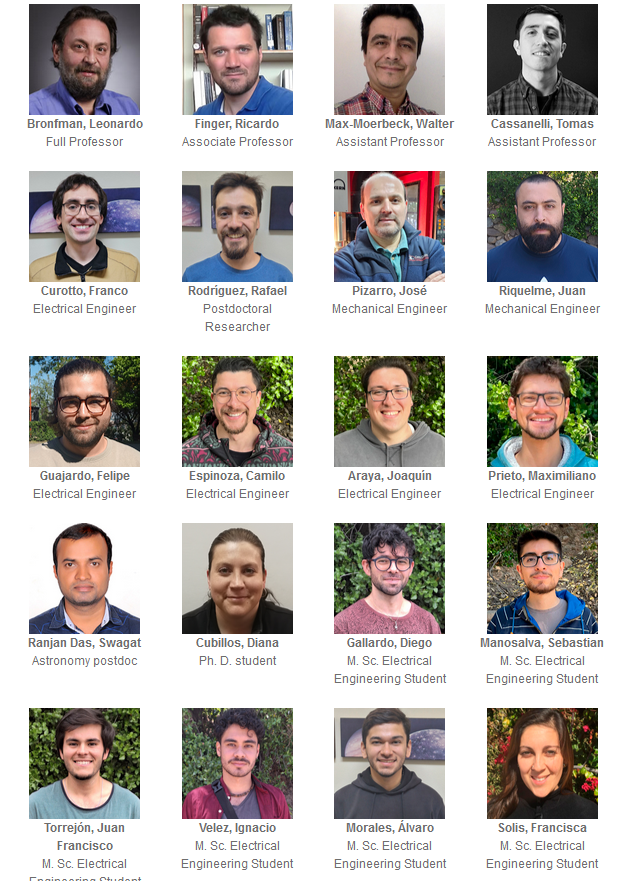
\includegraphics[width=0.6\textwidth]{ejemplos/Figura1.png}
	\caption{Ingenieros y estudiantes que son parte del laboratorio de ondas milimétricas.}
	\label{fig:personas_lab}
\end{figure}
Se realizaron trabajos asociados al  Proyecto CHART, cuyo principal objetivo es diseñar y optimizar un arreglo de antenas capaz de detectar aproximadamente 100 ráfagas rápidas de radio (FRBs) al año, dentro de un rango de frecuencias de 300 a 500 MHz, con un campo de visión de 90 grados. Este proyecto involucra tanto el desarrollo de prototipos de diversos componentes de Microondas, como el uso intensivo de simulaciones avanzadas (Por ejemplo los utilizados para simular pulsos de FRBS), optimización de parámetros y la integración de diversos elementos tecnológicos.\\\\
El trabajó a realizar consistio en el diseño y caracterizacion de una antena Log-Periodic Dipole Array (LPDA), la cual es ampliamente utilizada en radioastronomía y telecomunicaciones, conocida por su capacidad de operar en un amplio rango de frecuencias. La optimización de esta antena se enfocó en maximizar su ganancia y mejorar la adaptabilidad de su patrón de radiación, considerando diferentes factores clave.\\\\
La elección de esta práctica responde a mis intereses en el area de la intrumentacion astronomica, campos que requieren un dominio avanzado del diseño y optimización de sistemas de antenas como de simular, ademas del permitirme acercarme de mejor manera a las investigaciones y proyectos mas recientes. Esta experiencia me permitió colaborar de manera efectiva con otros profesionales, fortaleciendo sus capacidades de trabajo en equipo y el aprender a incorporar diferentes partes de un proyecto en un todo coherente.\\\\
\newpage
\section{Descripción general de la empresa u organización}
El Laboratorio de Ondas Milimétricas (MWL), perteneciente al Departamento de Astronomía y al Departamento de Ingeniería Eléctrica de la Universidad de Chile, se enfoca en el desarrollo tecnológico avanzado dentro del campo de la radioastronomía como se presento previamente. Desde su fundación, ha logrado consolidarse como un centro clave en la investigación científica y en la fabricación de equipos. El MWL está dentro del sector de investigación y desarrollo científico-tecnológico, particularmente en las áreas de radioastronomía y telecomunicaciones. Su trabajo abarca desde el diseño de receptores de ondas milimétricas hasta la optimización de antenas para la observación astronómica, colaborando con instituciones internacionales como por ejemplo con ALMA (\ref{fig:ALMA})y el Centro de Excelencia en Astrofísica y Tecnologías Afines (CATA) (\ref{fig:LLama}), entre otros.\\\\
\begin{figure}[H]
    \centering
    \subfloat[Visualización Conceptual del proyecto LLAMA, el cual corresponde a un radiotelescopio de 12 metros de diámetro.]{%
        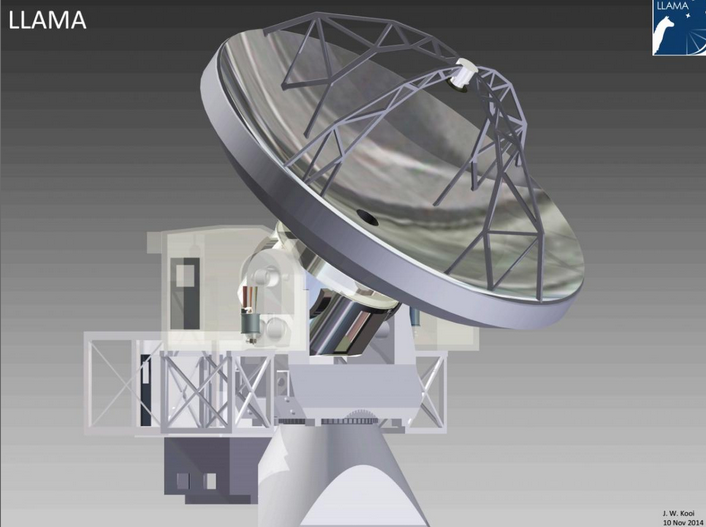
\includegraphics[width=0.5\textwidth]{ejemplos/Figura2.png}
        \label{fig:LLama}}
    \quad
    \subfloat[Horn utilizado para la banda 1 de ALMA, que opera entre 35 y 50 GHz.]{%
        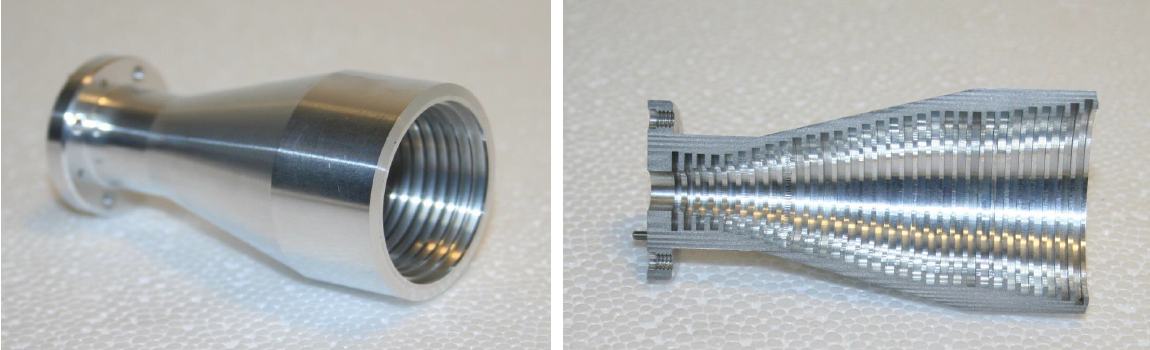
\includegraphics[width=0.5\textwidth]{ejemplos/Figure3.png}
        \label{fig:ALMA}}
    \caption{Contextualizacion de alunos proyectos de ejemplos llevado a cabo por el laboratorio de ondas milimetricas}
    \label{fig:example}
\end{figure}
La misión principal del laboratorio es diseñar, fabricar y optimizar  receptores de ondas milimétricas, entre mas aspectos,ademas del analisis y estudio de datos astronomicos, esto  con el fin de contribuir al avance de la ciencia y la tecnología en el ámbito astronómico.El MWL cuenta con un equipo multidisciplinario que incluye astrónomos, ingenieros, técnicos y estudiantes de pregrado y postgrado. Está dirigido por el profesor Ricardo Finger y Tomas Cassanelli, quienes son encargados de variados proyectos.
\newpage
\section{Descripción del trabajo realizado}
Como se menciono inicialmente, se realizaon trabajos en el marco del Proyecto CHART, el cual busca diseñar y optimizar un arreglo de antenas capaz de detectar ráfagas rápidas de radio (FRBs) en un rango de frecuencias de 300 a 500 MHz. En este contexto, se me fue asignada la tarea de diseñar y optimizar una antena Log-Periodic Dipole Array (LPDA).
\begin{figure}
	\centering
	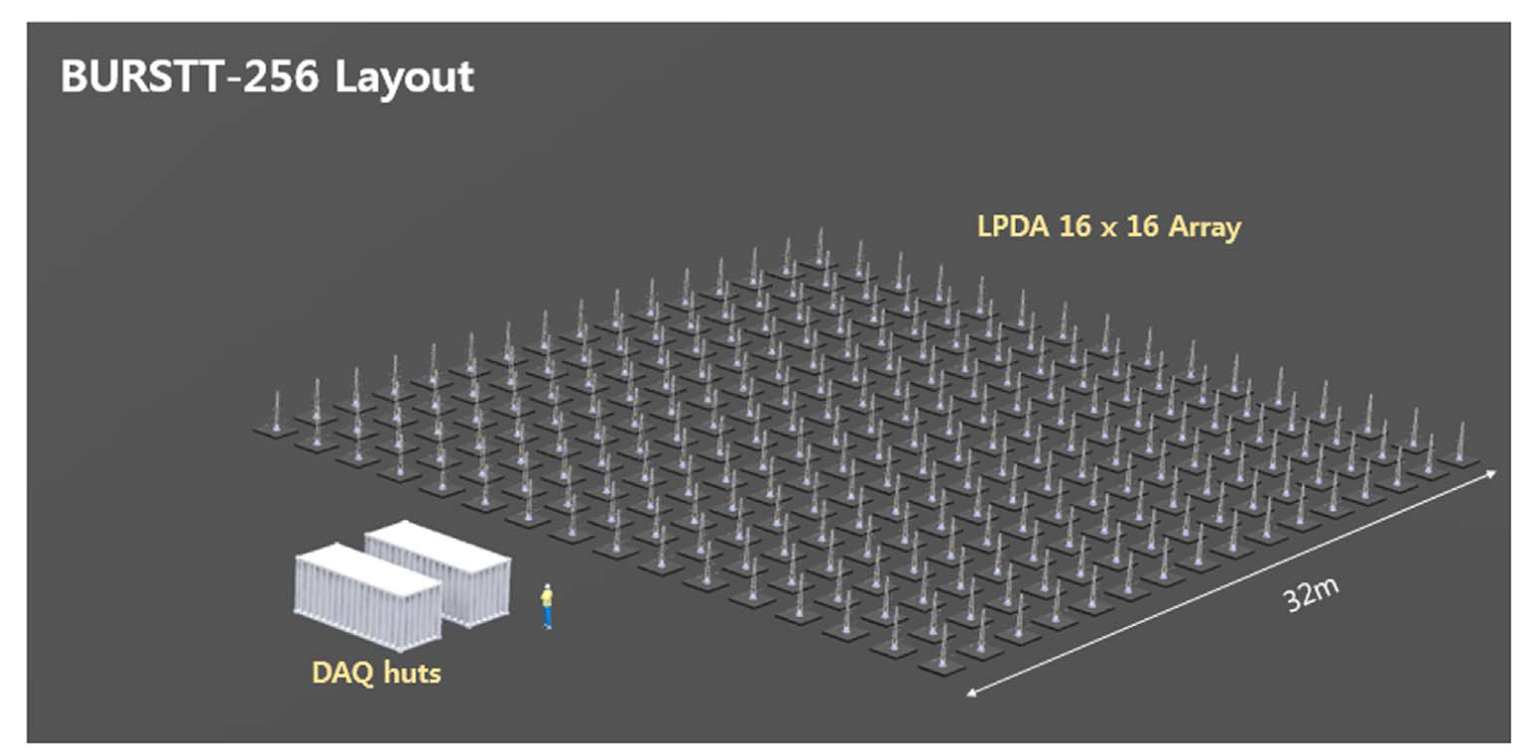
\includegraphics[width=0.7\textwidth]{ejemplos/Figure4.png}
	\caption{Esquema conceptual del Array de antenas a implementar para el proyecto CHART, donde se tendran un arreglo de 16x16, dando un total de 256 antenas.}
	\label{fig:personas_lab}
\end{figure}
Para el diseño e implementacion de la antena, se toma en consideracion el siguiente esquema general donde se observa una vista general de los diferentes elementos de interes. (\ref{fig:esquema_antena}),
donde se observan los parametros mas importantes a considera
\begin{figure}
	\centering
	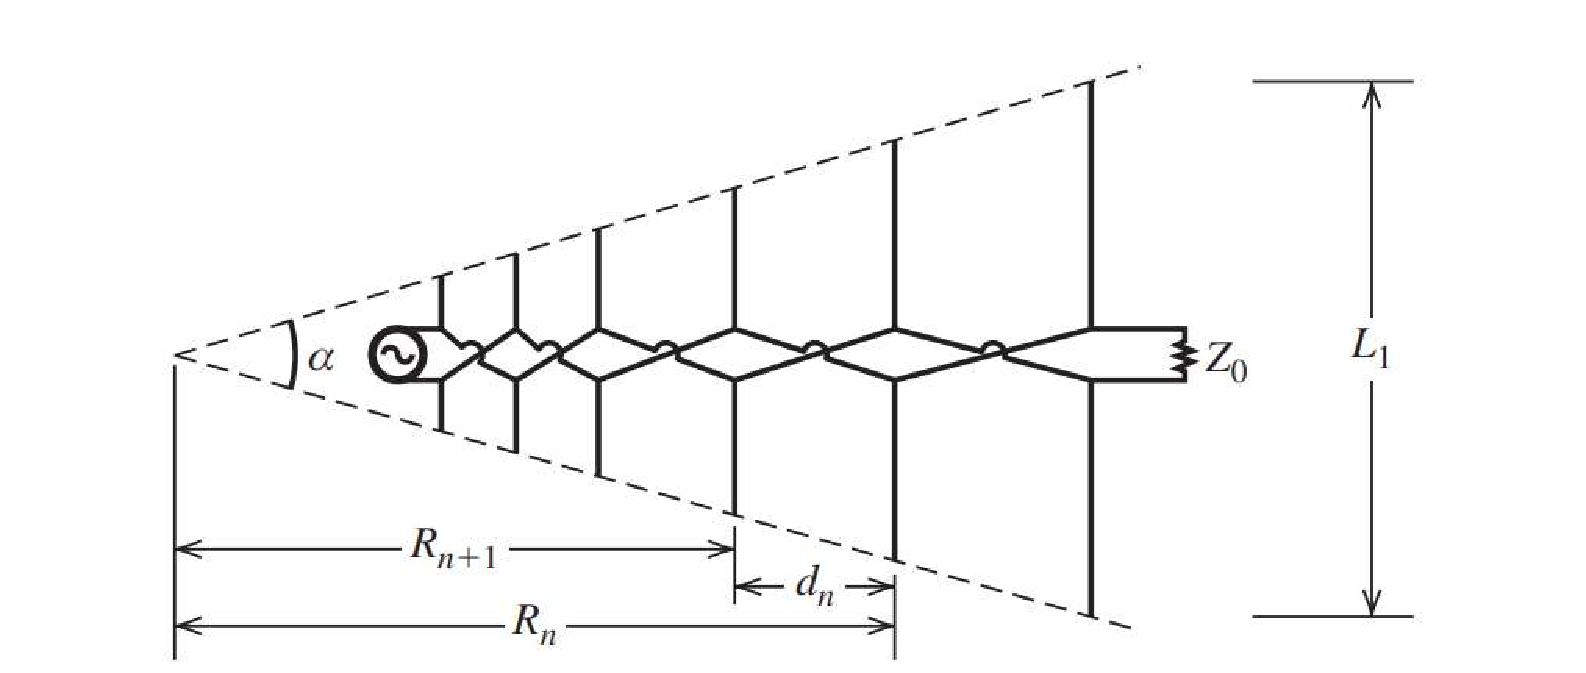
\includegraphics[width=0.8\textwidth]{ejemplos/Figure5.pdf}
	\caption{Descripción general de una antena LPDA, considerando parámetros clave como las distancias relativas entre los elementos \(d_n\), el ángulo \(\alpha\) que indica la apertura y distribución de los dipolos, la alimentación de la antena visible al principio y, finalmente, las longitudes \(L_n\). (Stutzman \& Thiele 1997)}
	\label{fig:esquema_antena}
\end{figure}
Dos parámetros críticos, \(\tau\) y \(\sigma\), son tomados en cuenta, donde el primero está asociado a la relación entre los diferentes elementos de la antena, y el segundo corresponde al espaciamiento relativo. La selección de ambos parámetros es arbitraria, con el objetivo de optimizar una ganancia máxima y se realiza mediante el grafico adjunto \ref{fig:Parametros_antena}
\begin{figure}
	\centering
	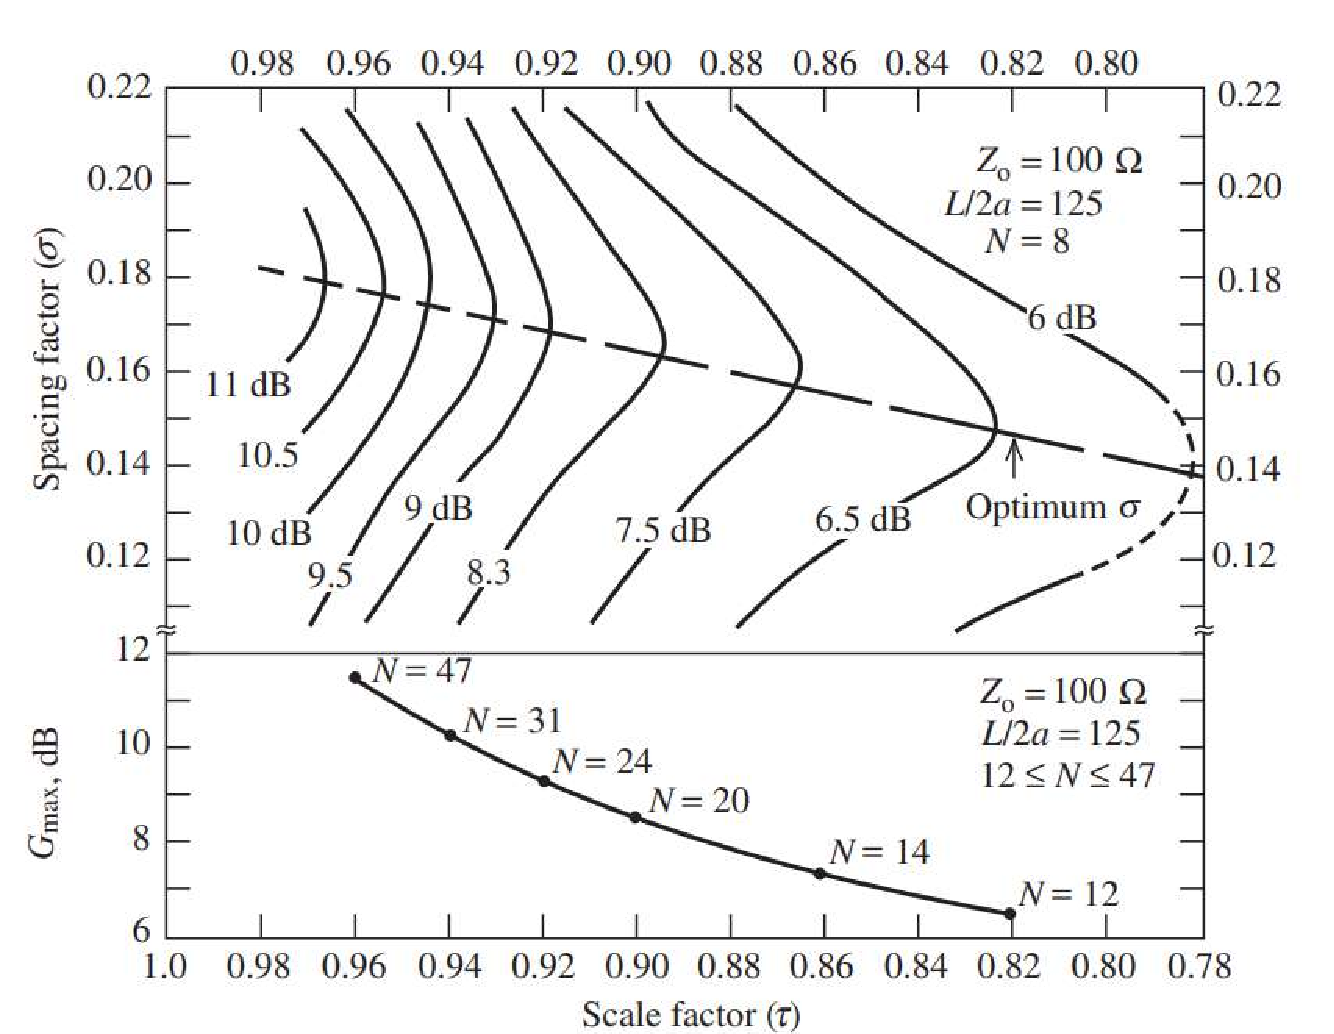
\includegraphics[width=0.6\textwidth]{ejemplos/Figure6.pdf}
	\caption{Espacio relativo $\sigma$ en funcion del parametro $\tau$ para una  LPDA, es importante destacar ademas, que el grafico inferior corresponde a el crecimiento exponencial en el numero de elementos que se deben adicionar en caso de buscar mas ganancia y por tanto una mayor directividad}
	\label{fig:Parametros_antena}
\end{figure}
\begin{figure}
	\centering
	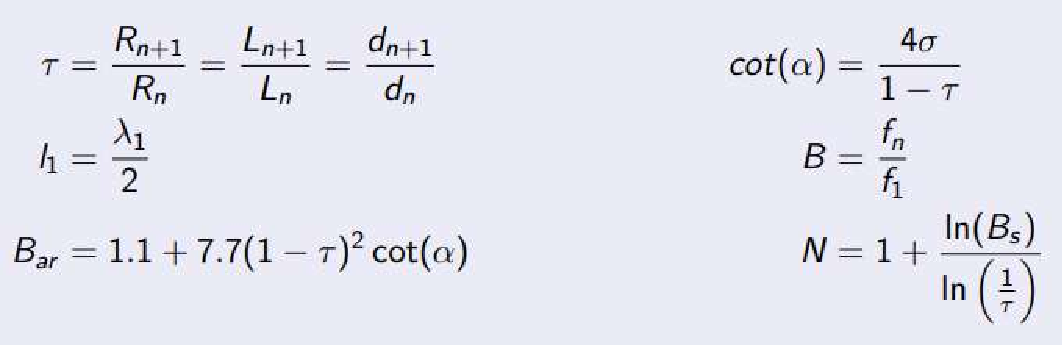
\includegraphics[width=0.7\textwidth]{ejemplos/Figure7.pdf}
	\caption{Algunas de las ecuaciones importantes que permiten obtener la cantidad de elementos necesarios para una LPDA, ademas de otras caracteristicas como la relacion entre elemento y elemento.}
	\label{fig:esqumea_antena}
\end{figure}
Posteriormente se hace uso del software \textit{HFSS} (el cual corresponde a un simulador electromagnético basado en el método de elementos finitos), donde se procedió a parametrizar y optimizar las diferentes variables que caracterizan a la antena, dando como lo mesjores valores los vistos en la tabla a continuacion \ref{tab:Parametros_optimizados}:
\begin{table}
    \captionsetup{position=below}
    \footnotesize
    \label{tab:antenna-parameters11}
    \begin{subtable}[b]{0.45\linewidth}
        \centering
        \begin{tabular}{cc}
            \multicolumn{2}{c}{Elements for the LPDA antenna} \\
            \hline
            Frequency Range & 300 -- 500MHz \\
            Input Impedance & 50[$\Omega$] \\
            Square side of BOOM & 20 mm \\
            Elements diameter & 9.525 mm \\
            BOOM and dipoles material & Aluminum \\
            Gap material & Wood \\
            Aluminum bolts & -1.25 x 40 mm \\
            BOOM gap & 11.5 mm \\
            BOOM length & 1266 mm \\
            BOOM back & 124 mm \\
            $\tau$ & 0.9 \\
            $\sigma$ & 0.168 (Optimal) \\
            N & 11 \\
        \end{tabular}
        \caption{Valores seleccionados para la fabricación de la antena}
        \label{tab:caracteristicas_generales}
    \end{subtable}%
    \hspace{1cm} % Agrega espacio entre las dos tablas
    \begin{subtable}[b]{0.45\linewidth}
        \centering
        \begin{tabular}{cccc}
            \multicolumn{4}{c}{Dipole lengths and distances} \\
            \hline
            L1 & 243 mm & $D_{1 \rightarrow 2}$ & 174 mm \\
            L2 & 218 mm & $D_{2 \rightarrow 3}$ & 156 mm \\
            L3 & 194 mm & $D_{3 \rightarrow 4}$ & 141 mm \\
            L4 & 173 mm & $D_{4 \rightarrow 5}$ & 127 mm \\
            L5 & 155 mm & $D_{5 \rightarrow 6}$ & 114 mm \\
            L6 & 138 mm & $D_{6 \rightarrow 7}$ & 103 mm \\
            L7 & 122 mm & $D_{7 \rightarrow 8}$ & 92 mm \\
            L8 & 109 mm & $D_{8 \rightarrow 9}$ & 83 mm \\
            L9 & 96 mm & $D_{9 \rightarrow 10}$ & 75 mm \\
            L10 & 85 mm & $D_{10 \rightarrow 11}$ & 67 mm \\
            L11 & 75 mm & - & - \\
        \end{tabular}
        \caption{Largos de los dipolos como distancia entre ellos}
        \label{tab:Parametros_optimizados}
    \end{subtable}
\end{table}
Se tomo en consideracion todo lo anterior, ademas de variados detalles que permiten acercarse de mejor manera a la realidad por sobre la simulacion en cuanto a distribucion de corrientes por ejemplo, la adicion de tornillos que sujetaran a los dipolos y el hecho de que los elementos son huecos(Se visualiza en \ref{fig:vistas_antena}).
\begin{figure}[H]
    \centering
    \subfloat[Vista frontal de la LPDA, que permite observar las consideraciones tomadas para la simulacion, como las varillas de aluminio y el BOOM hueco, asi como la consideracion de los tornillos, que son relevantes en terminos de adaptacion.]{%
        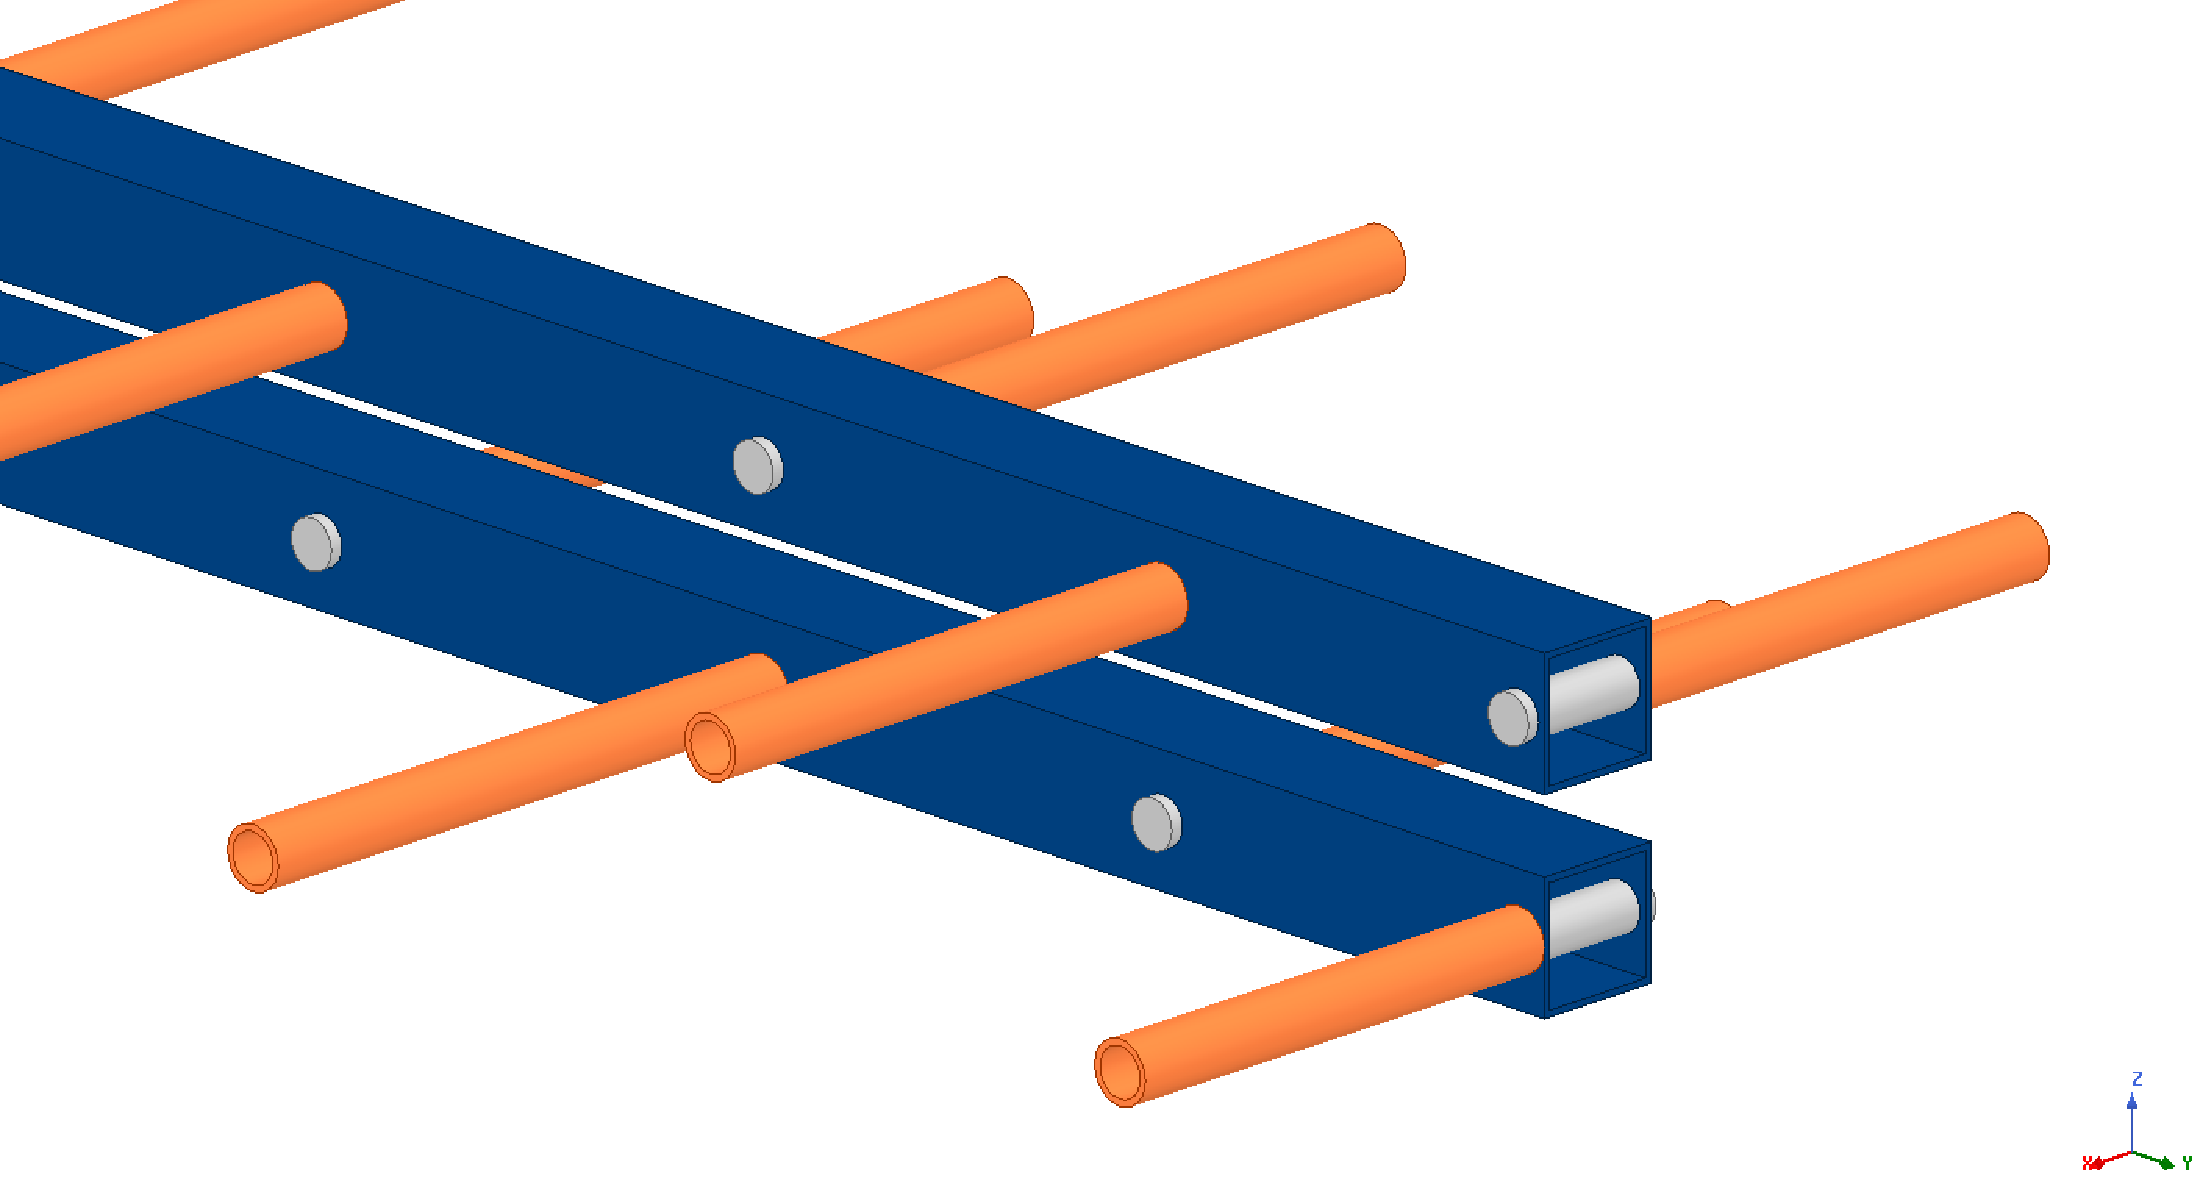
\includegraphics[width=0.4\textwidth]{ejemplos/Figure8.pdf}
        \label{fig:y-equals-x}}
    \quad
    \subfloat[Vista superior de la antena LPDA para observar caracteristicas de medicion, como la separacion entre los dipolos]{%
        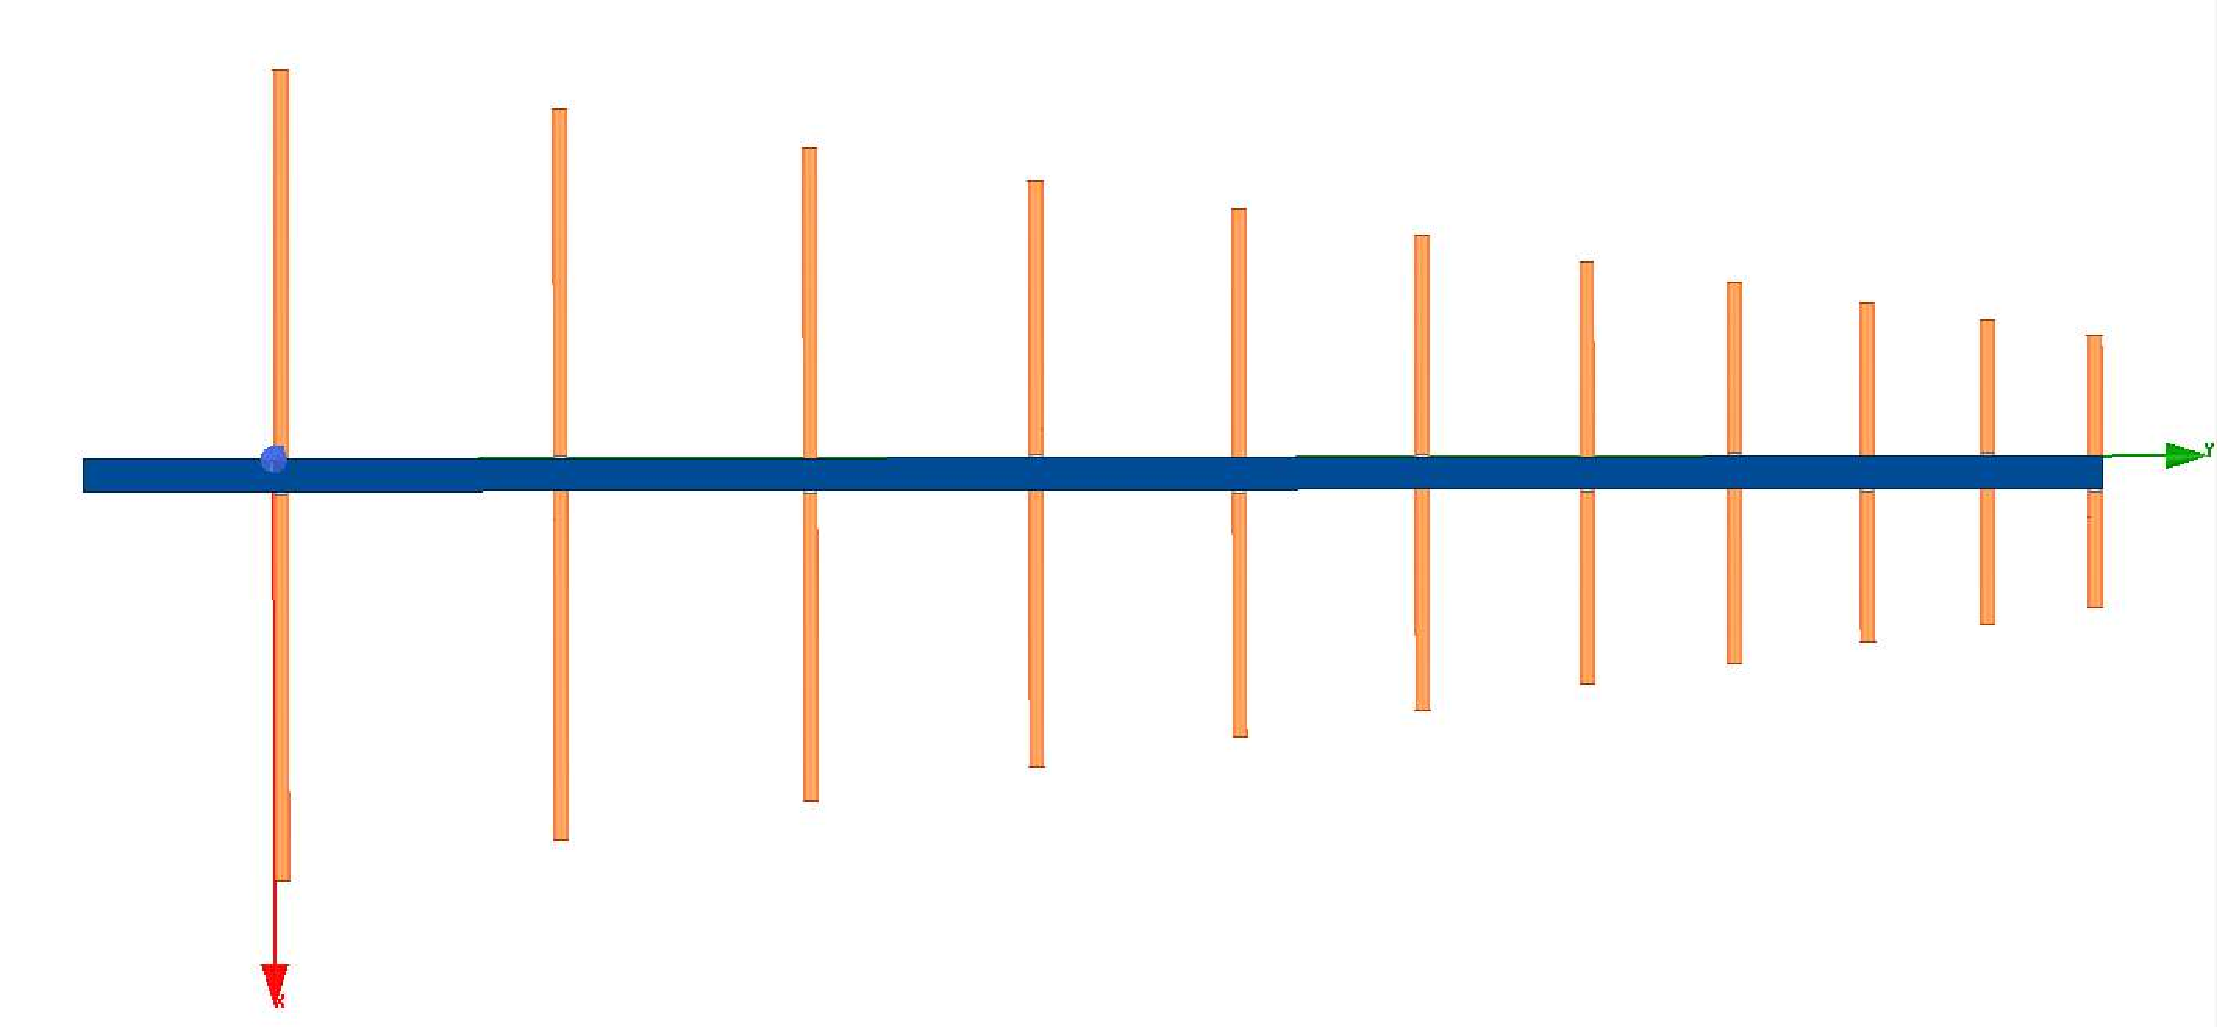
\includegraphics[width=0.4\textwidth]{ejemplos/Figure9.pdf}
        \label{fig:three-sin-x}}
    \caption{Vista isometrica y superior de la antena LPDA, donde se observan las consideraciones tomadas para la simulacion y la fabricacion de la antena.}
    \label{fig:vistas_antena}
\end{figure}
Una vez considerado todo lo anterior se tiene que el $E - Plane$ y el $H - Plane$ viene dado por lo siguiente (Se realiza para un rango de frecuencias desde 300 -- 500 Mhz, el cual es el rango de interes para el proyecto CHART):
\begin{figure}
	\centering
	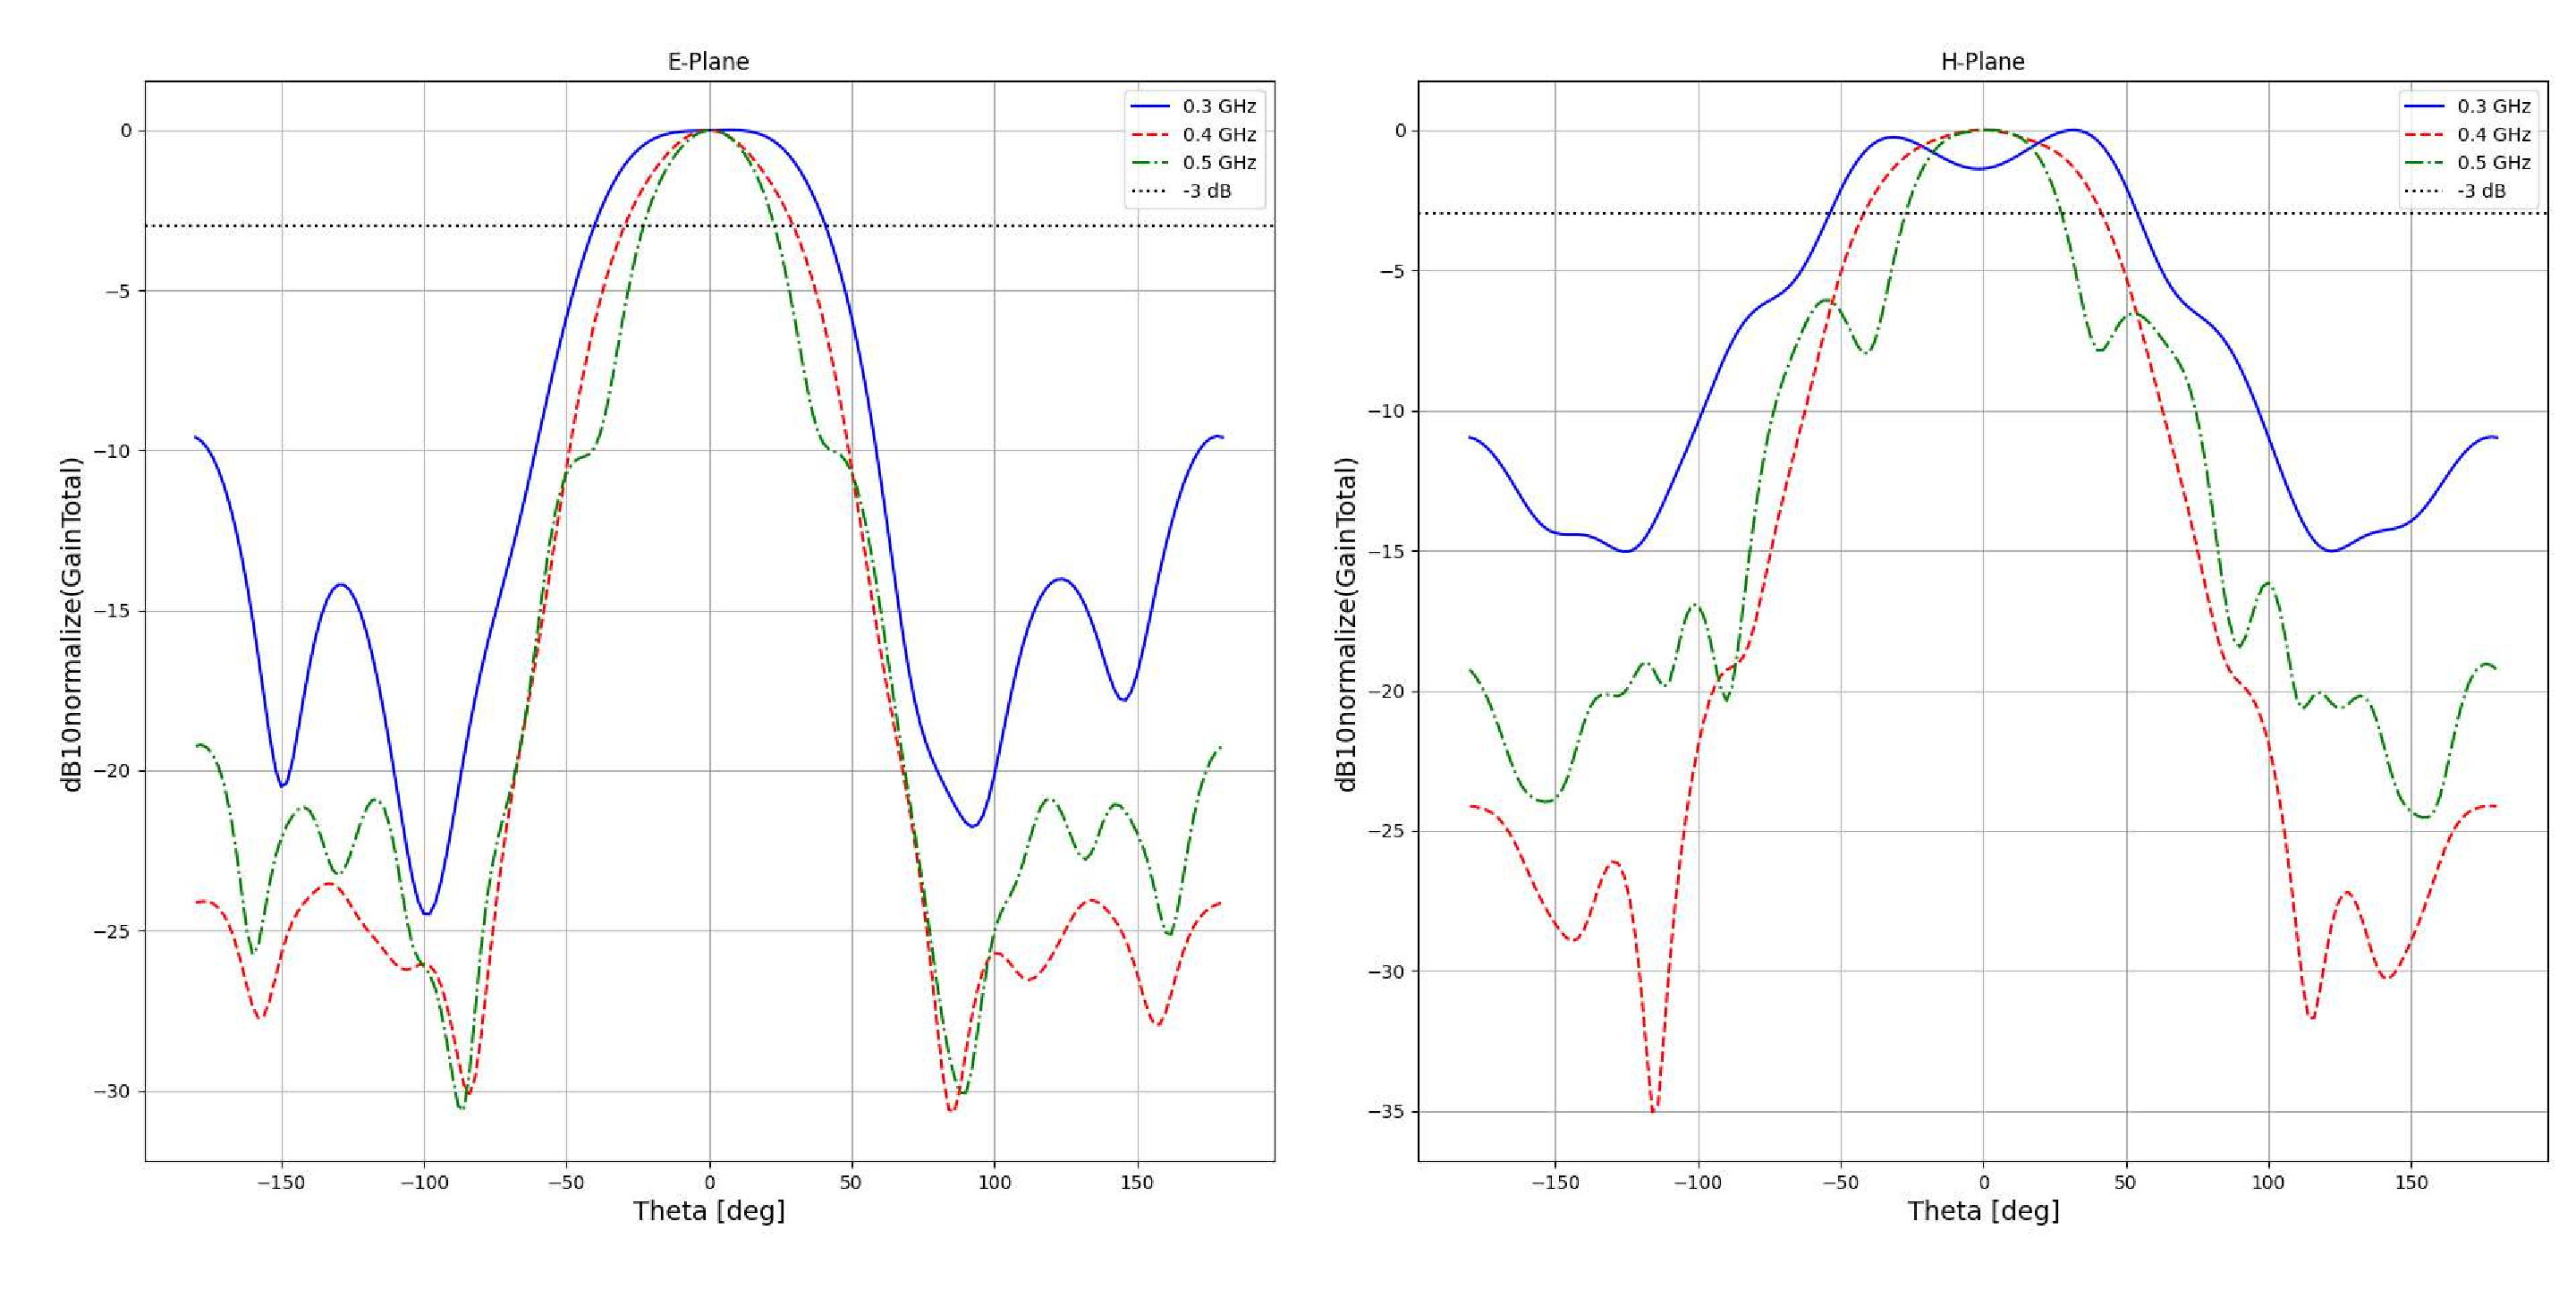
\includegraphics[width=1.1\textwidth]{ejemplos/Figure10.pdf }
	\caption{Ganancia normalizada en funcion del angulo (grados). Esto se realiza para los planos E y H, permitiendo el analisis
	del campo de vision (FOV) asi como la distribucion espacial del patron de radiacion, para frecuencias de 300 MHz, 400
	MHz y 500 MHz, cubriendo el ancho de banda de interes.}
	\label{fig:esqumea_antena}
\end{figure}
Se resume los valores obtenidos en cuanto a el HPBW (Half Power Beam Width) (\ref{tab:lpda_beamwidth}), asi como los valores de los materiales utilizados para la fabricacion de la antena (\ref{tab:Materials_LPDA}).
  \begin{table}
      \centering
      \begin{tabular}{|c|c|c|c|}
          \hline
          & 300MHz & 400MHz & 500MHz \\
          \hline
          Plano E & 81.1$^{\circ}$   &  60$^{\circ}$ & 46$^{\circ}$ \\
          Plano H & 111.04$^{\circ}$  & 83$^{\circ}$  & 55$^{\circ}$ \\
          \hline
      \end{tabular}
      \caption{Patrón de radiación}
      \label{tab:lpda_beamwidth}
  \end{table}
    \begin{table}[H]
      \centering
      \caption{Materiales utilizados en la construcción de la antena LPDA}
      \label{tab:Materials_LPDA}
      \begin{tabular}{|l|l|l|}
          \hline
          \textbf{Material} & \textbf{Descripción} & \textbf{Costo (USD)} \\ \hline
          Perfiles de aluminio & Dos perfiles (25mm x 25mm), longitud total 1.3m & 20.34 \\ \hline
          Barras de aluminio & Seis barras (diámetro de 3/8 pulgadas), longitud total 6m & 15.32 \\ \hline
          Pernos & 50 pernos P.HEX.DIN 933 (H-T) INOX.A2 M8-1.25 x 40 & 11.93 \\ \hline
      \end{tabular}
  \end{table}
  Por lo tanto, se obtuvo un valor aproximado de \$47.59 USD, lo que permite la producción de aproximadamente 2 prototipos (considerando solo elementos esenciales y excluyendo herramientas ya disponibles en el taller donde fue fabricado). Posteriormente se tiene el primer prototipo el cual se visualiza en lo siguiente:
  \begin{figure}[H]
    \centering
    \subfloat[Vista frontal del prototipo de la LPDA, mostrando la caracterizacion de sus dipolos y sus distancias.]{%
        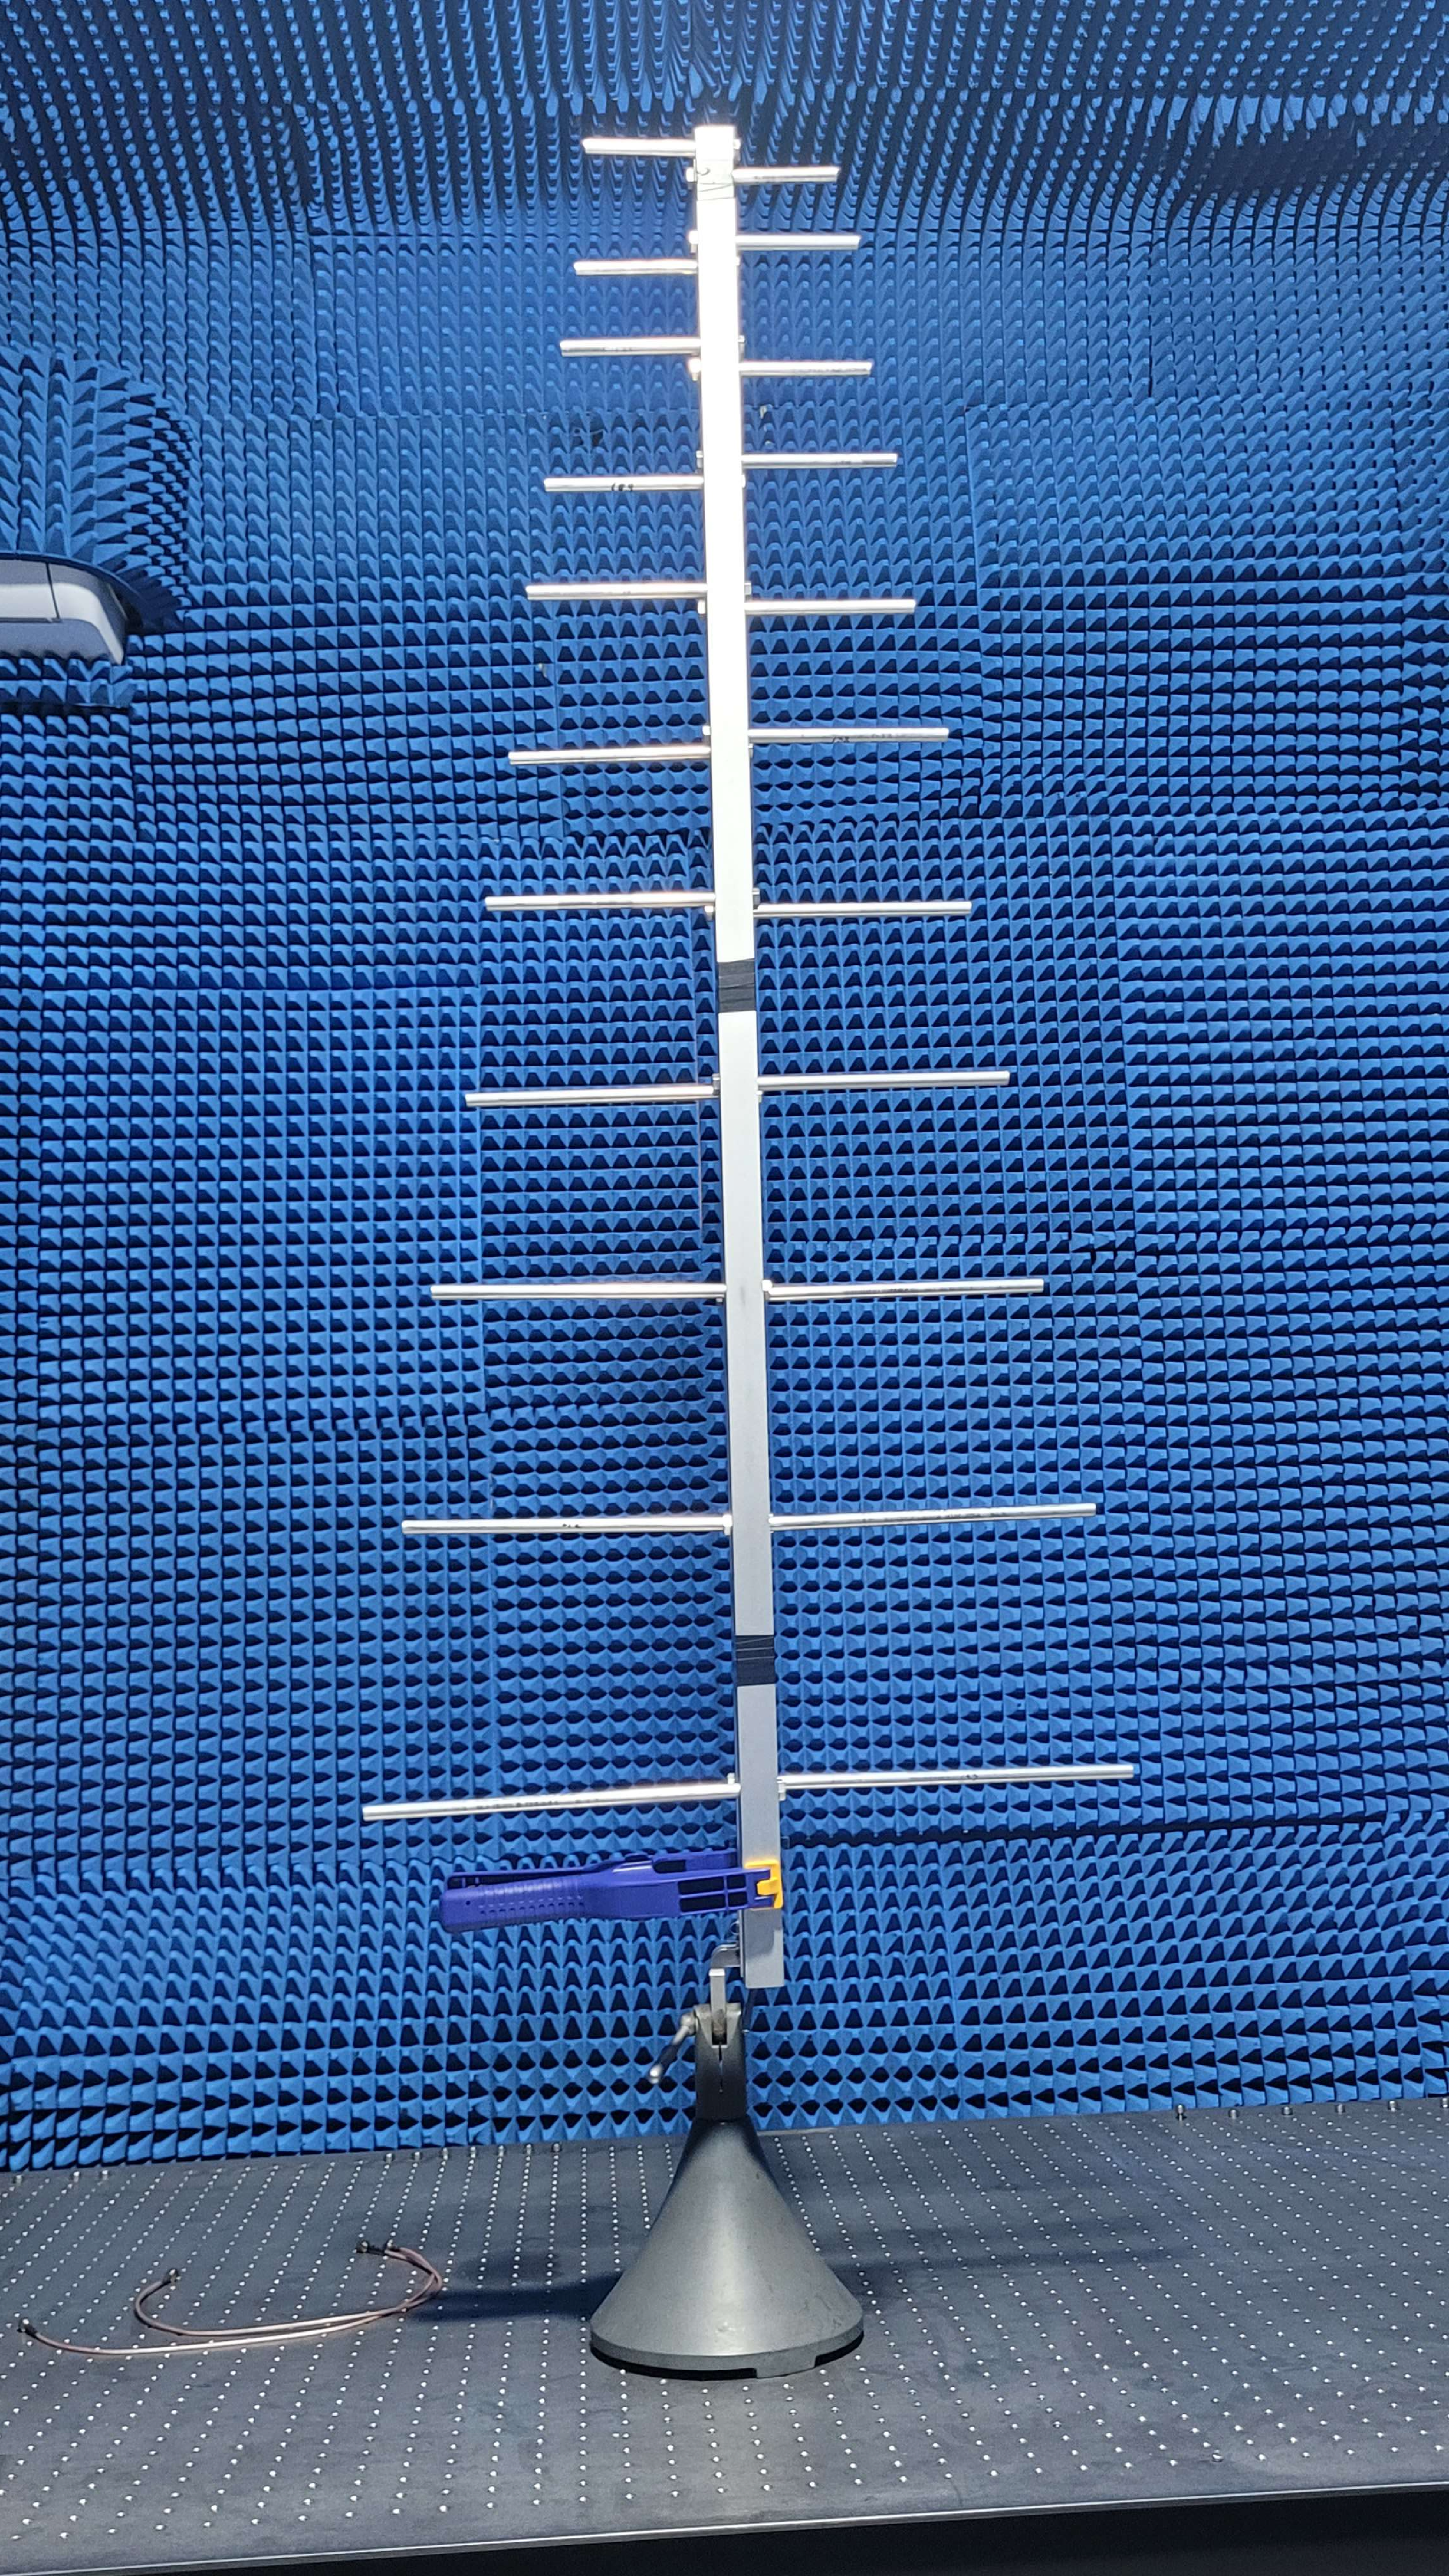
\includegraphics[width=0.25\textwidth]{ejemplos/Figure11.pdf}
        \label{fig:y-equals-x}}
    \quad
    \subfloat[Metodo utilizado para conectar los BOOMs, junto con los pernos observados]{%
        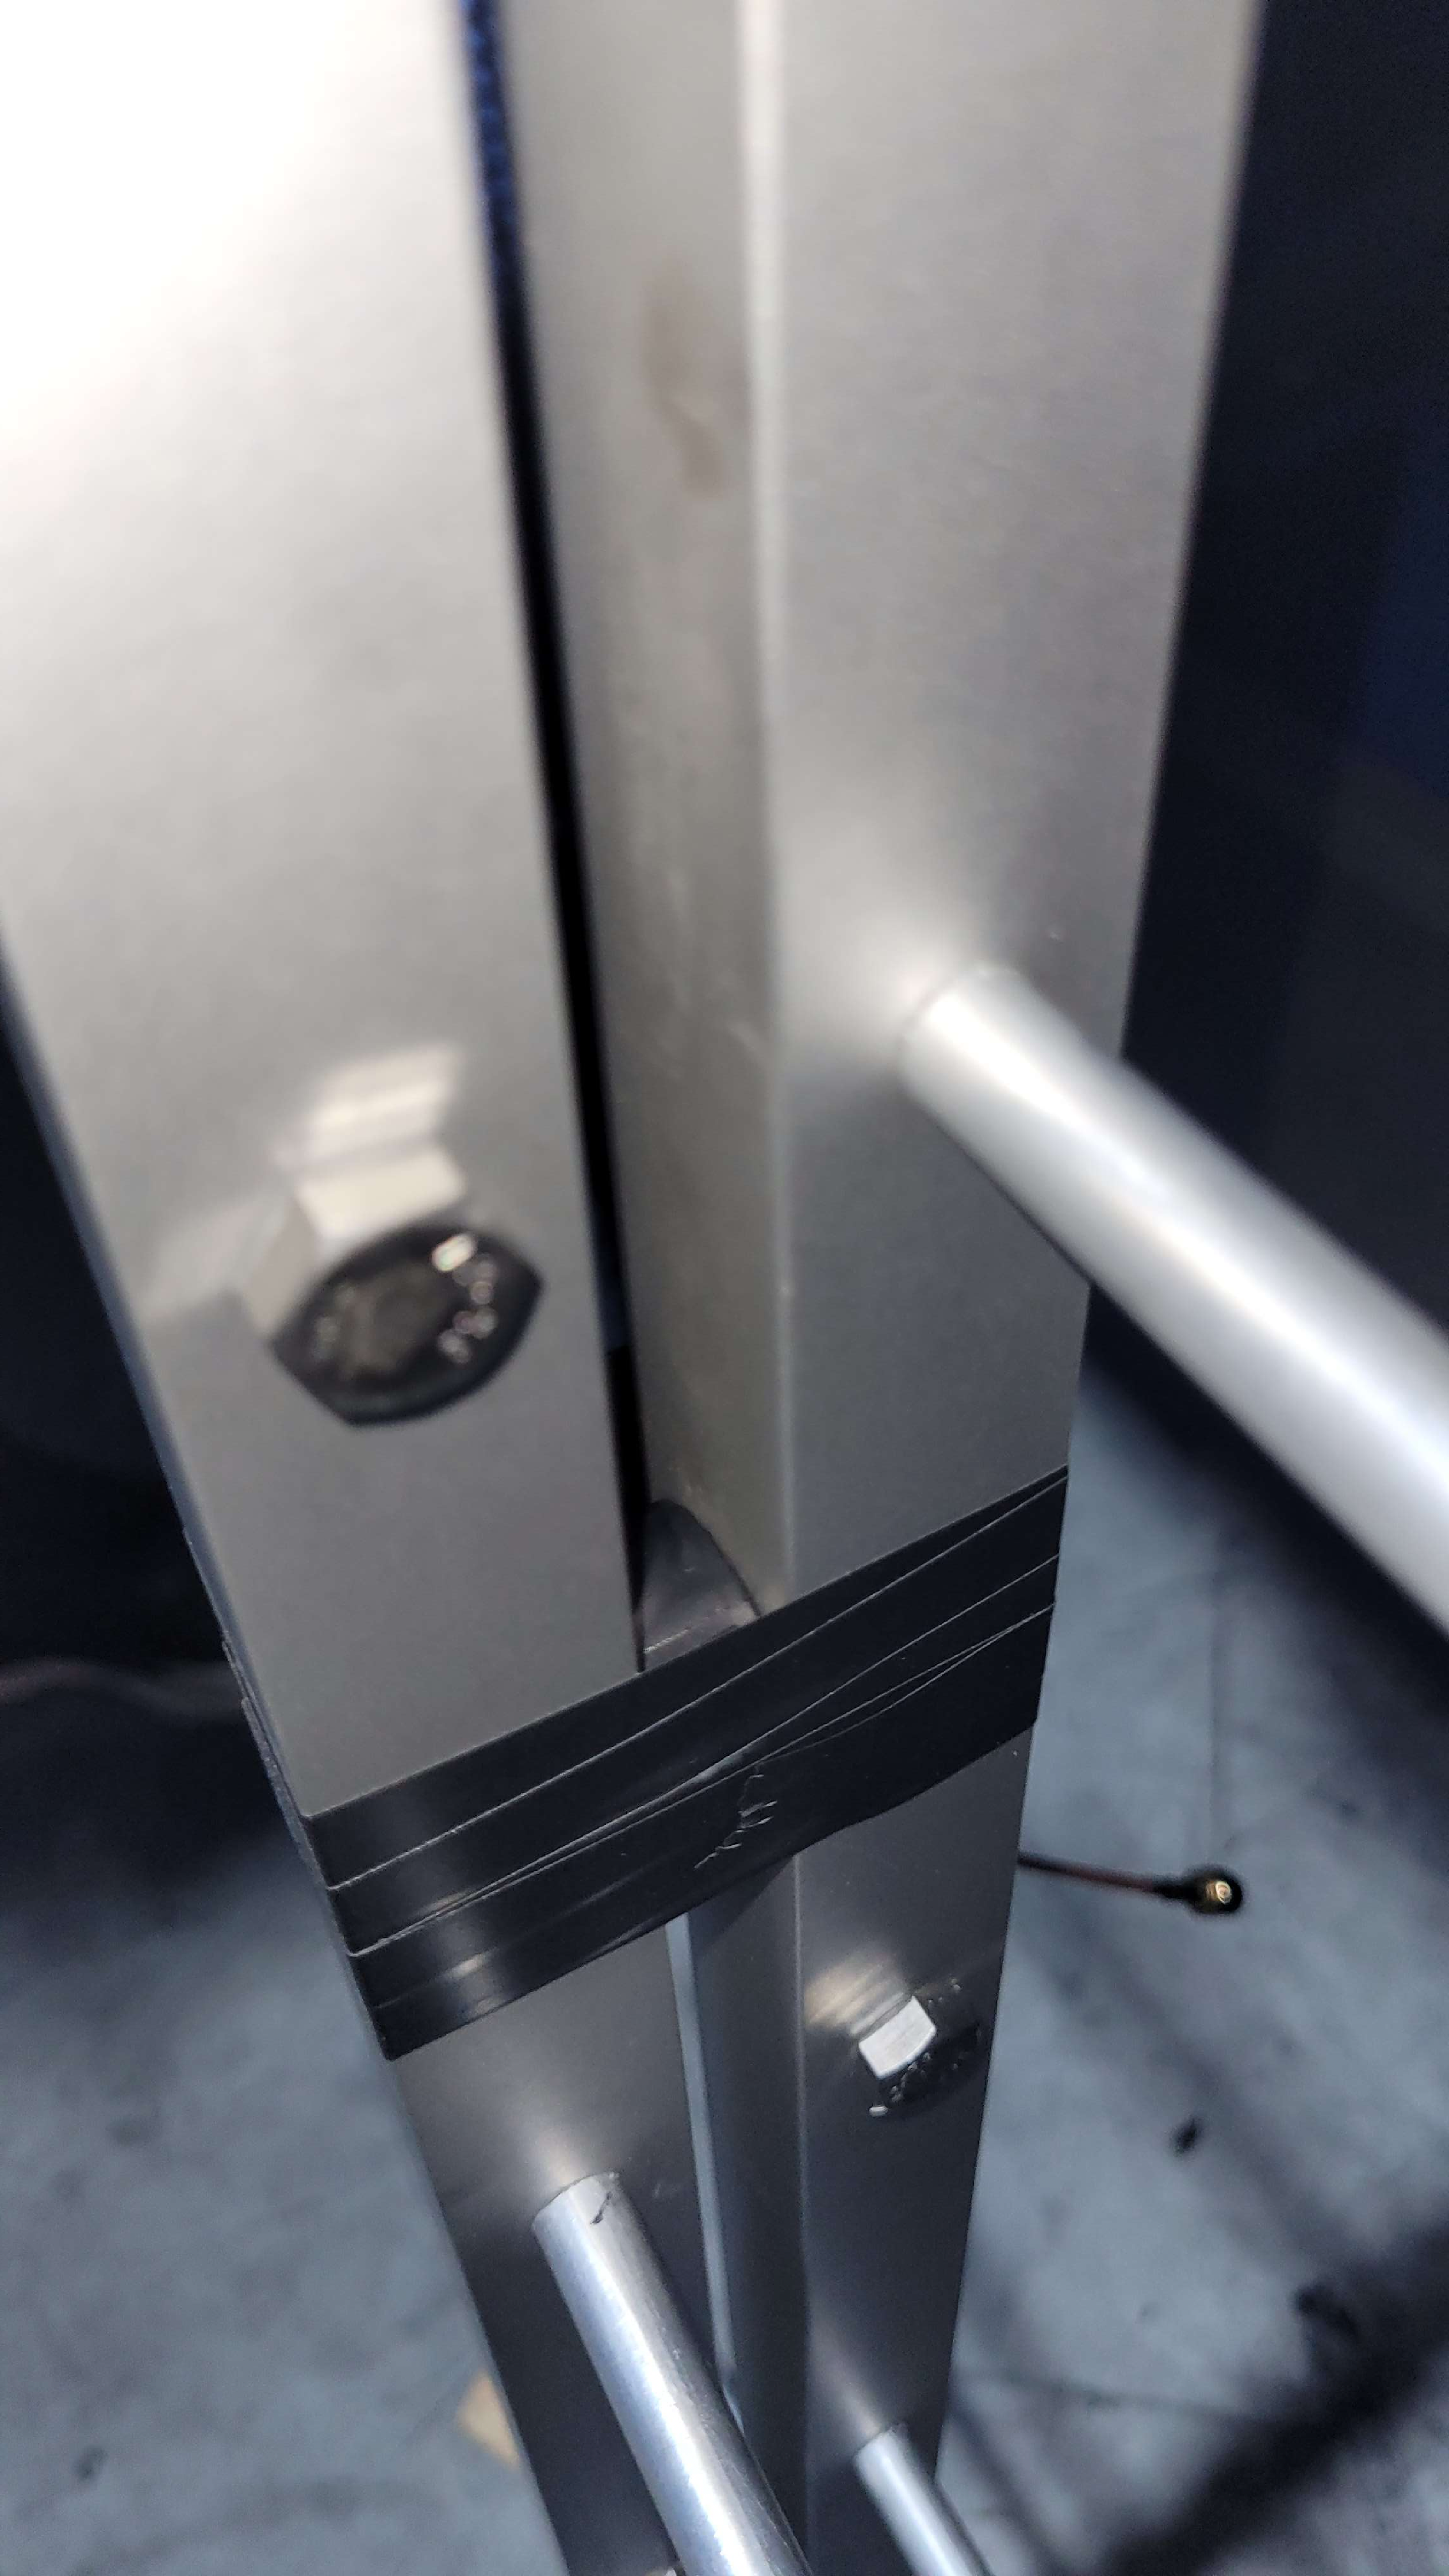
\includegraphics[width=0.25\textwidth]{ejemplos/Figure12.pdf}
        \label{fig:three-sin-x}}
    \caption{Vistas del primer prototipo realizado, donde se observa todos los aspectos considerados en la simulacion}
    \label{fig:example}
\end{figure}
Posteriormente se realizaron mediciones para ver su desempeño en cuanto a las reflexiones o equivalentemente su parametro $S_{11}$ dando como resultado lo siguiente:
\begin{figure}
	\centering
	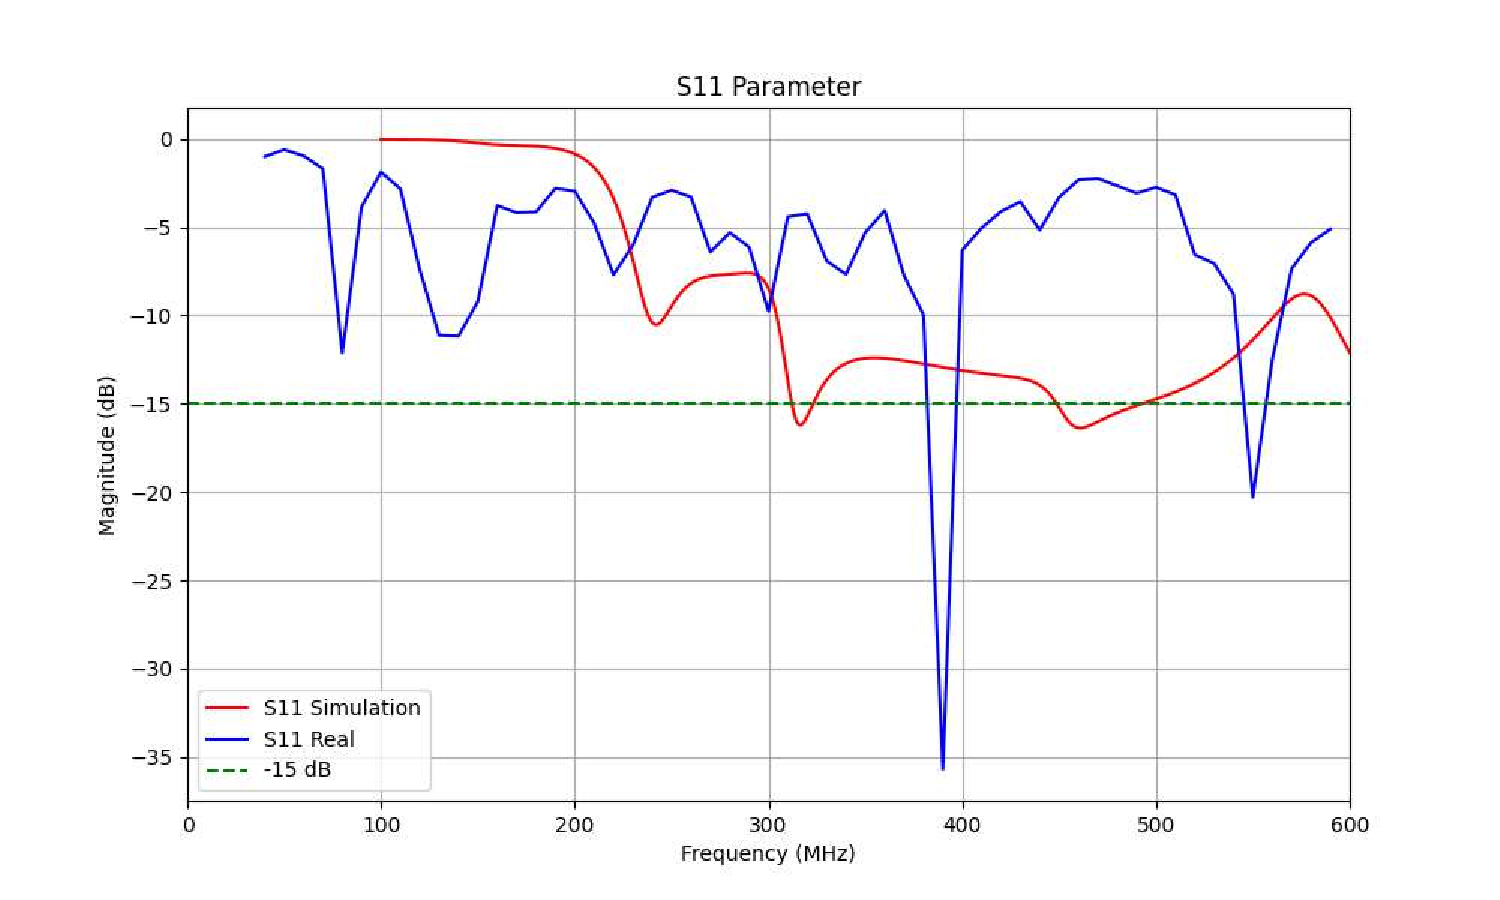
\includegraphics[width=0.7\textwidth]{ejemplos/Figure18.pdf}
	\caption{Comparacion entre el parametro S11 simulado (rojo) y el parametro S11 obtenido del VNA (azul). Se obtienen resultados deficientes para las mediciones pero esto se debe a la conexion, lo cual se resolvera en futuras iteraciones}
	\label{fig:esqumea_antena}
\end{figure}
\begin{figure}
	\centering
	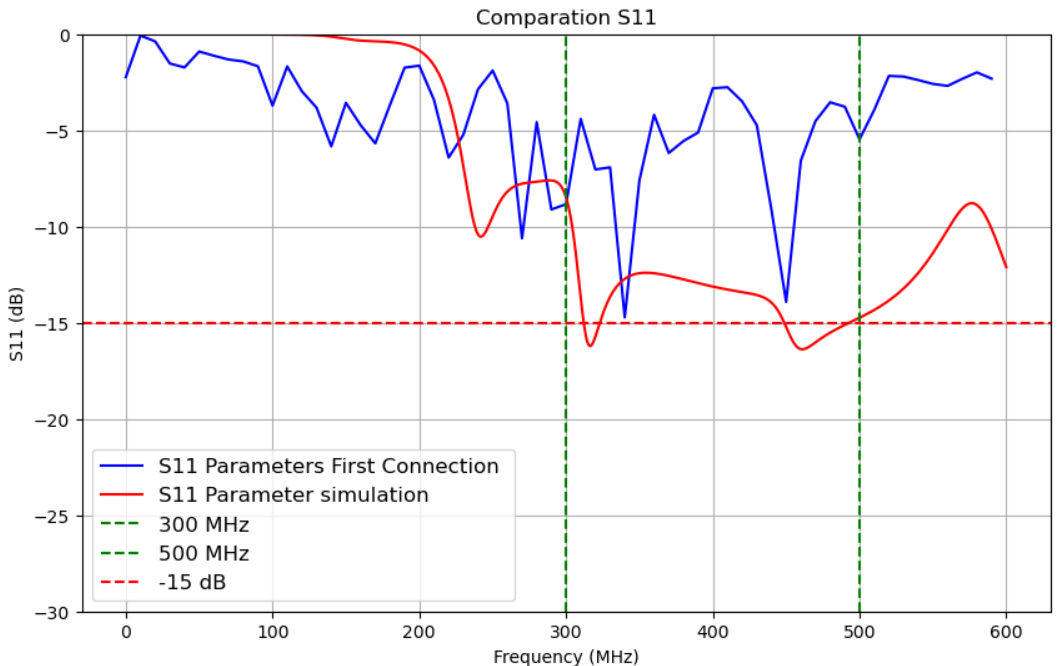
\includegraphics[width=0.7\textwidth]{ejemplos/Figure13.png}
	\caption{Se realizó un cambio en la conexión, implementándose mediante un perno en cada cara interna del BOOM, lo que permitió que se asemejara más a la simulación}
	\label{fig:esqumea_antena}
\end{figure}
\begin{figure}
	\centering
	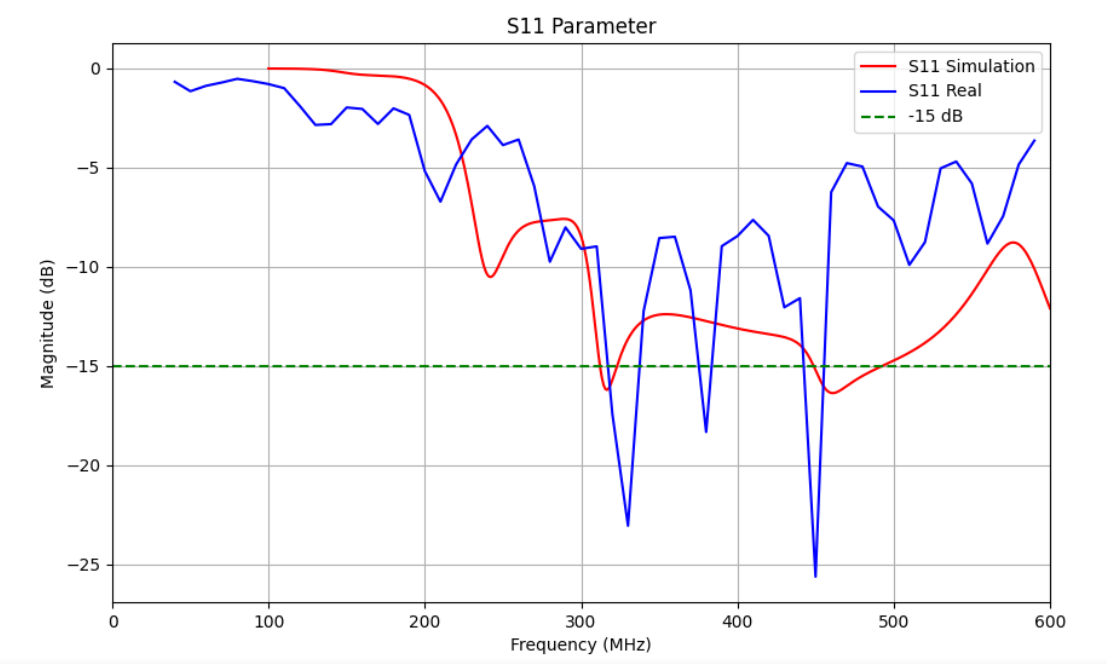
\includegraphics[width=0.7\textwidth]{ejemplos/Figure14.png}
	\caption{Se mantuvo la conexión anterior, pero se cambió el valor del GAP a 7.5 mm, siendo este el valor óptimo. Como se mencionó anteriormente, este parámetro mejora significativamente la adaptación de la antena.}
	\label{fig:esqumea_antena}
\end{figure}
\begin{figure}
	\centering
	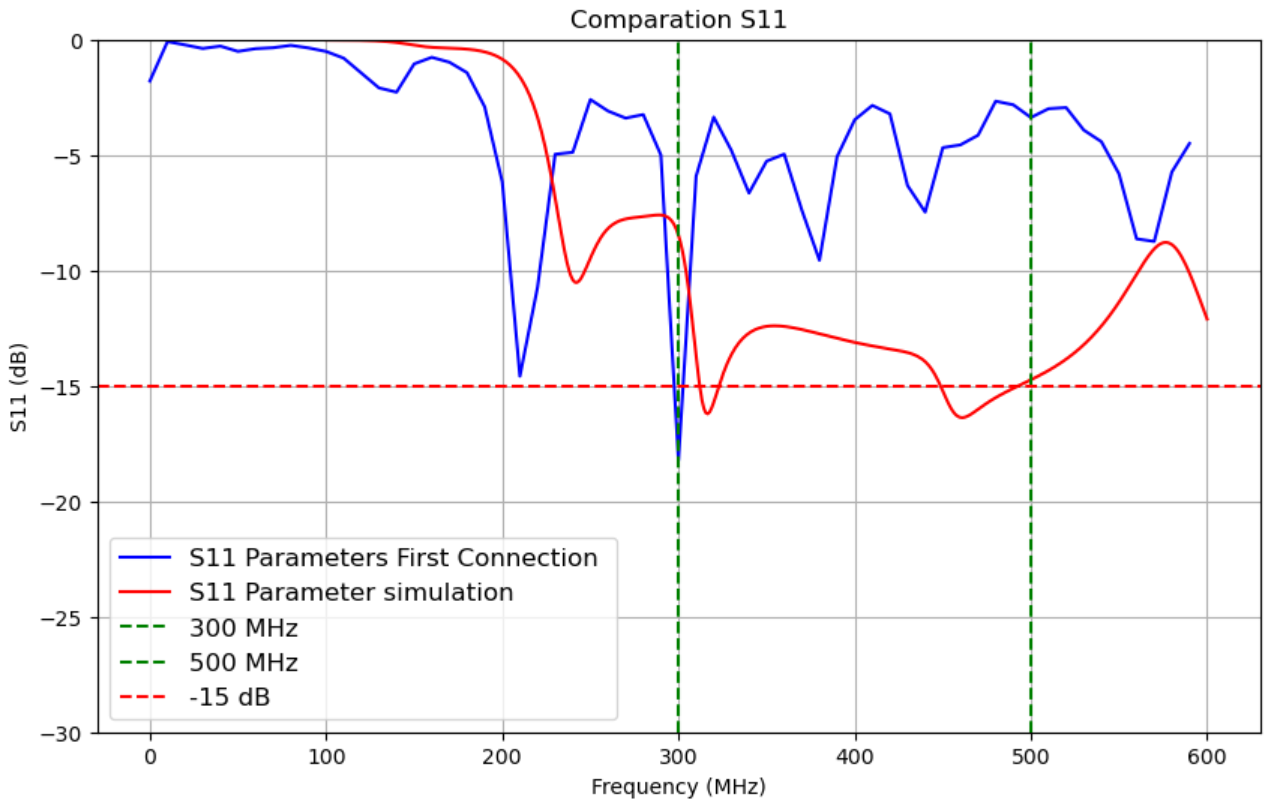
\includegraphics[width=0.7\textwidth]{ejemplos/Figure15.png}
	\caption{La conexión se mejoró implementando una línea Microstrip, lo que permitió una distribución de corriente más uniforme a lo largo de las caras internas del BOOM. Además, se eliminó la extensión del BOOM que anteriormente se utilizaba para conectar mediante los pernos, haciéndolo más similar a la simulación.}
	\label{fig:esqumea_antena}
\end{figure}
Finalmente se observo una buena respuesta con el tercer tipo de conexion en la antena. Se realiza una comparación con los resultados obtenidos en BURSTT, que muestran prometedores respuestas para el modelo. Sin embargo, es esencial considerar que el orden de magnitud aún está en desarrollo, ya que planeamos incorporar el parámetro de Medida de Dispersión (DM).
\begin{figure}[H]
    \centering
    \subfloat[Grafico de area efectiva, FOV y SEFD medido en Janksy para prototipo de CHART.]{%
        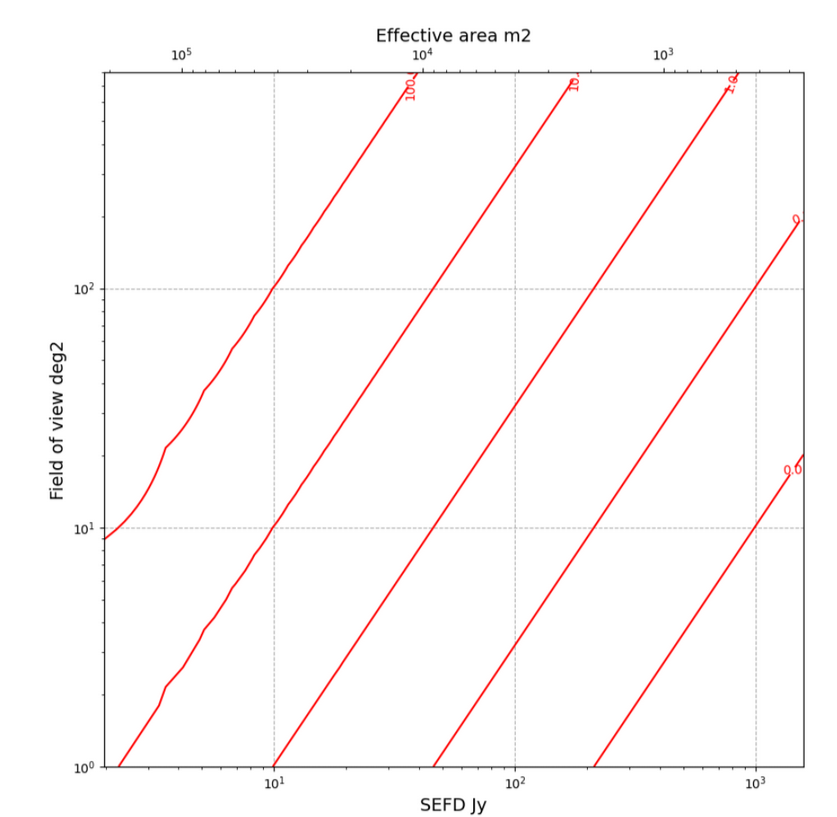
\includegraphics[width=0.5\textwidth]{ejemplos/Figure16.png}
        \label{fig:y-equals-x}}
    \quad
    \subfloat[Horn utilizado para la banda 1 de ALMA, que opera entre 35 y 50 GHz.]{%
        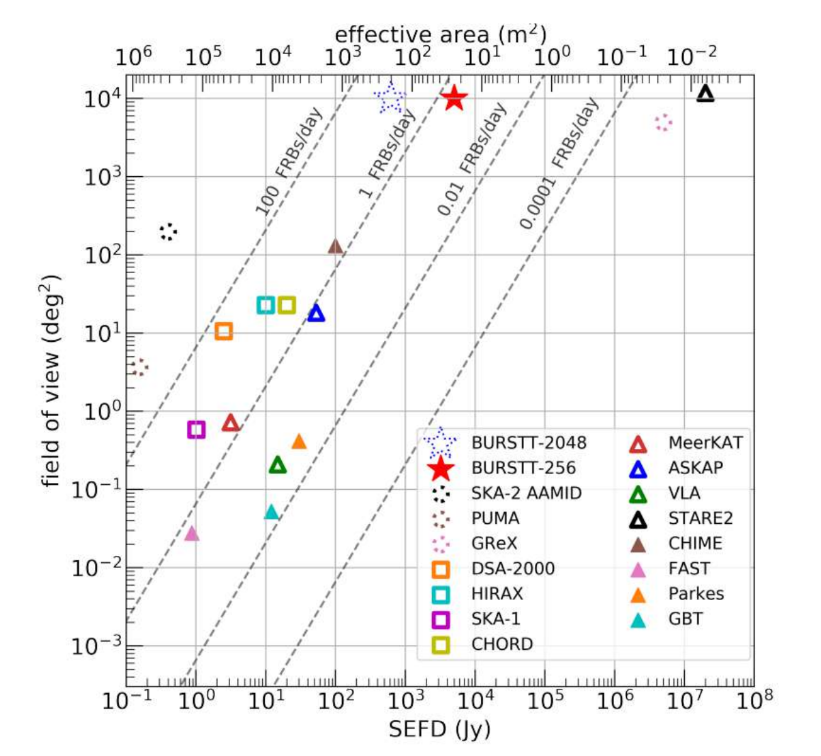
\includegraphics[width=0.55\textwidth]{ejemplos/Figure17.png}
        \label{fig:three-sin-x}}
    \caption{Grafico de area efectiva, FOV y SEFD medido en Janksy para BURSTT}
    \label{fig:example}
\end{figure}
El equipo en el cual se participó fue el grupo de trabajo AstroLabs, compuesto por aproximadamente ocho integrantes, cada uno con funciones diferenciadas pero trabajando de manera conjunta en el proyecto CHART. Por ejemplo, algunos miembros estaban enfocados en la simulación de pulsos FRBs, que luego serían utilizados para evaluar la eficacia de la antena, mientras que otros se encargaban de la red de multiplexadores y otros componentes, como los amplificadores de bajo ruido (LNA). Esto exigía una comunicación constante entre los integrantes de las distintas áreas del proyecto.\\

En cuanto a las fortalezas y debilidades identificadas durante la práctica, se destacan las siguientes:
\begin{enumerate}
    \item \textbf{Fortalezas:} Se contaba con un conocimiento previo en el área y en el manejo de software de simulación, lo que permitió una rápida adaptación al proyecto CHART. Además, la capacidad de trabajo en equipo y la disposición para aprender de los demás integrantes resultaron fundamentales para el desarrollo del proyecto.
    \item \textbf{Debilidades:} La falta de experiencia en la fabricación de antenas condujo a cometer errores en la conexión de la antena, los cuales se pudieron solucionar con la colaboración de los otros integrantes del equipo. Asimismo, en diversas ocasiones no se mantuvo una comunicación adecuada con el resto del grupo, debido a una excesiva concentración en el trabajo individual.
\end{enumerate}
\newpage
\section{Análisis crítico del proceso de práctica}
Durante la realización de la práctica profesional, se adquirieron diversos aprendizajes tanto en el ámbito profesional como en el personal. En el aspecto profesional, se desarrolló un dominio significativo en el uso de herramientas de simulación como HFSS, lo que permitió optimizar de manera eficiente el diseño de la Log-Periodic Dipole Array (LPDA). También se adquirieron habilidades clave en el análisis realista de antenas y la evaluación de patrones de radiación. En el ámbito personal, la colaboración con profesionales y estudiantes dentro del equipo AstroLabs fomentó tanto la capacidad de trabajo en equipo como la comunicación efectiva entre las distintas áreas del proyecto. Además, esta experiencia en un proyecto investigativo real ha proporcionado una base sólida para abordar futuros proyectos con mayor seguridad y eficiencia.\\

Respecto a la formación como Ingeniero Eléctrico en la FCFM, se identifican tanto fortalezas como debilidades:

\begin{enumerate}
    \item \textbf{Fortalezas:} La formación impartida por la FCFM proporciona una sólida base en matemáticas y física, junto con una capacidad crítica de análisis y resolución de problemas. Estas habilidades resultaron esenciales para abordar desafíos técnicos complejos y proponer soluciones efectivas. Además, el desarrollo de habilidades blandas permitió una mejor interacción dentro del equipo de trabajo, facilitando la adaptación a entornos colaborativos y multidisciplinarios.
    \item \textbf{Debilidades:} Se identificó una carencia de conocimientos avanzados en el área de instrumentación, lo cual se atribuye a la limitada oferta de cursos y profesores especializados en esta área específica. Este déficit tuvo que ser abordado de manera autodidacta durante la práctica, lo que resaltó la necesidad de ampliar la formación en esta área dentro del currículum académico.
\end{enumerate}
Finalmente, los aportes realizados a la organización incluyeron no solo el diseño optimizado de la antena LPDA, sino también una mejora en la coordinación y comunicación entre los distintos integrantes del proyecto, lo que contribuyó al éxito del mismo.
\newpage
\section{Referencia}
\begin{enumerate}
    \item W. L. Stutzman and G. A. Thiele, \textit{Antenna Theory and Design}. John Wiley \& Sons, 2nd ed., 1997.
    \item D. M. Pozar, \textit{Microwave Engineering}. John Wiley \& Sons, 4th ed., 2011.
    \item Astronomy Laboratory, ``Laboratorio de Astronomía,'' \url{https://astronomy-laboratory.github.io/index_spanish.html}, [Accessed: Oct. 14, 2024].
    \item Laboratorio de Ondas Milimétricas - Universidad de Chile, ``MWL Project,'' \url{http://www.das.uchile.cl/lab_mwl/project.html}, [Accessed: Oct. 14, 2024].
\end{enumerate}
